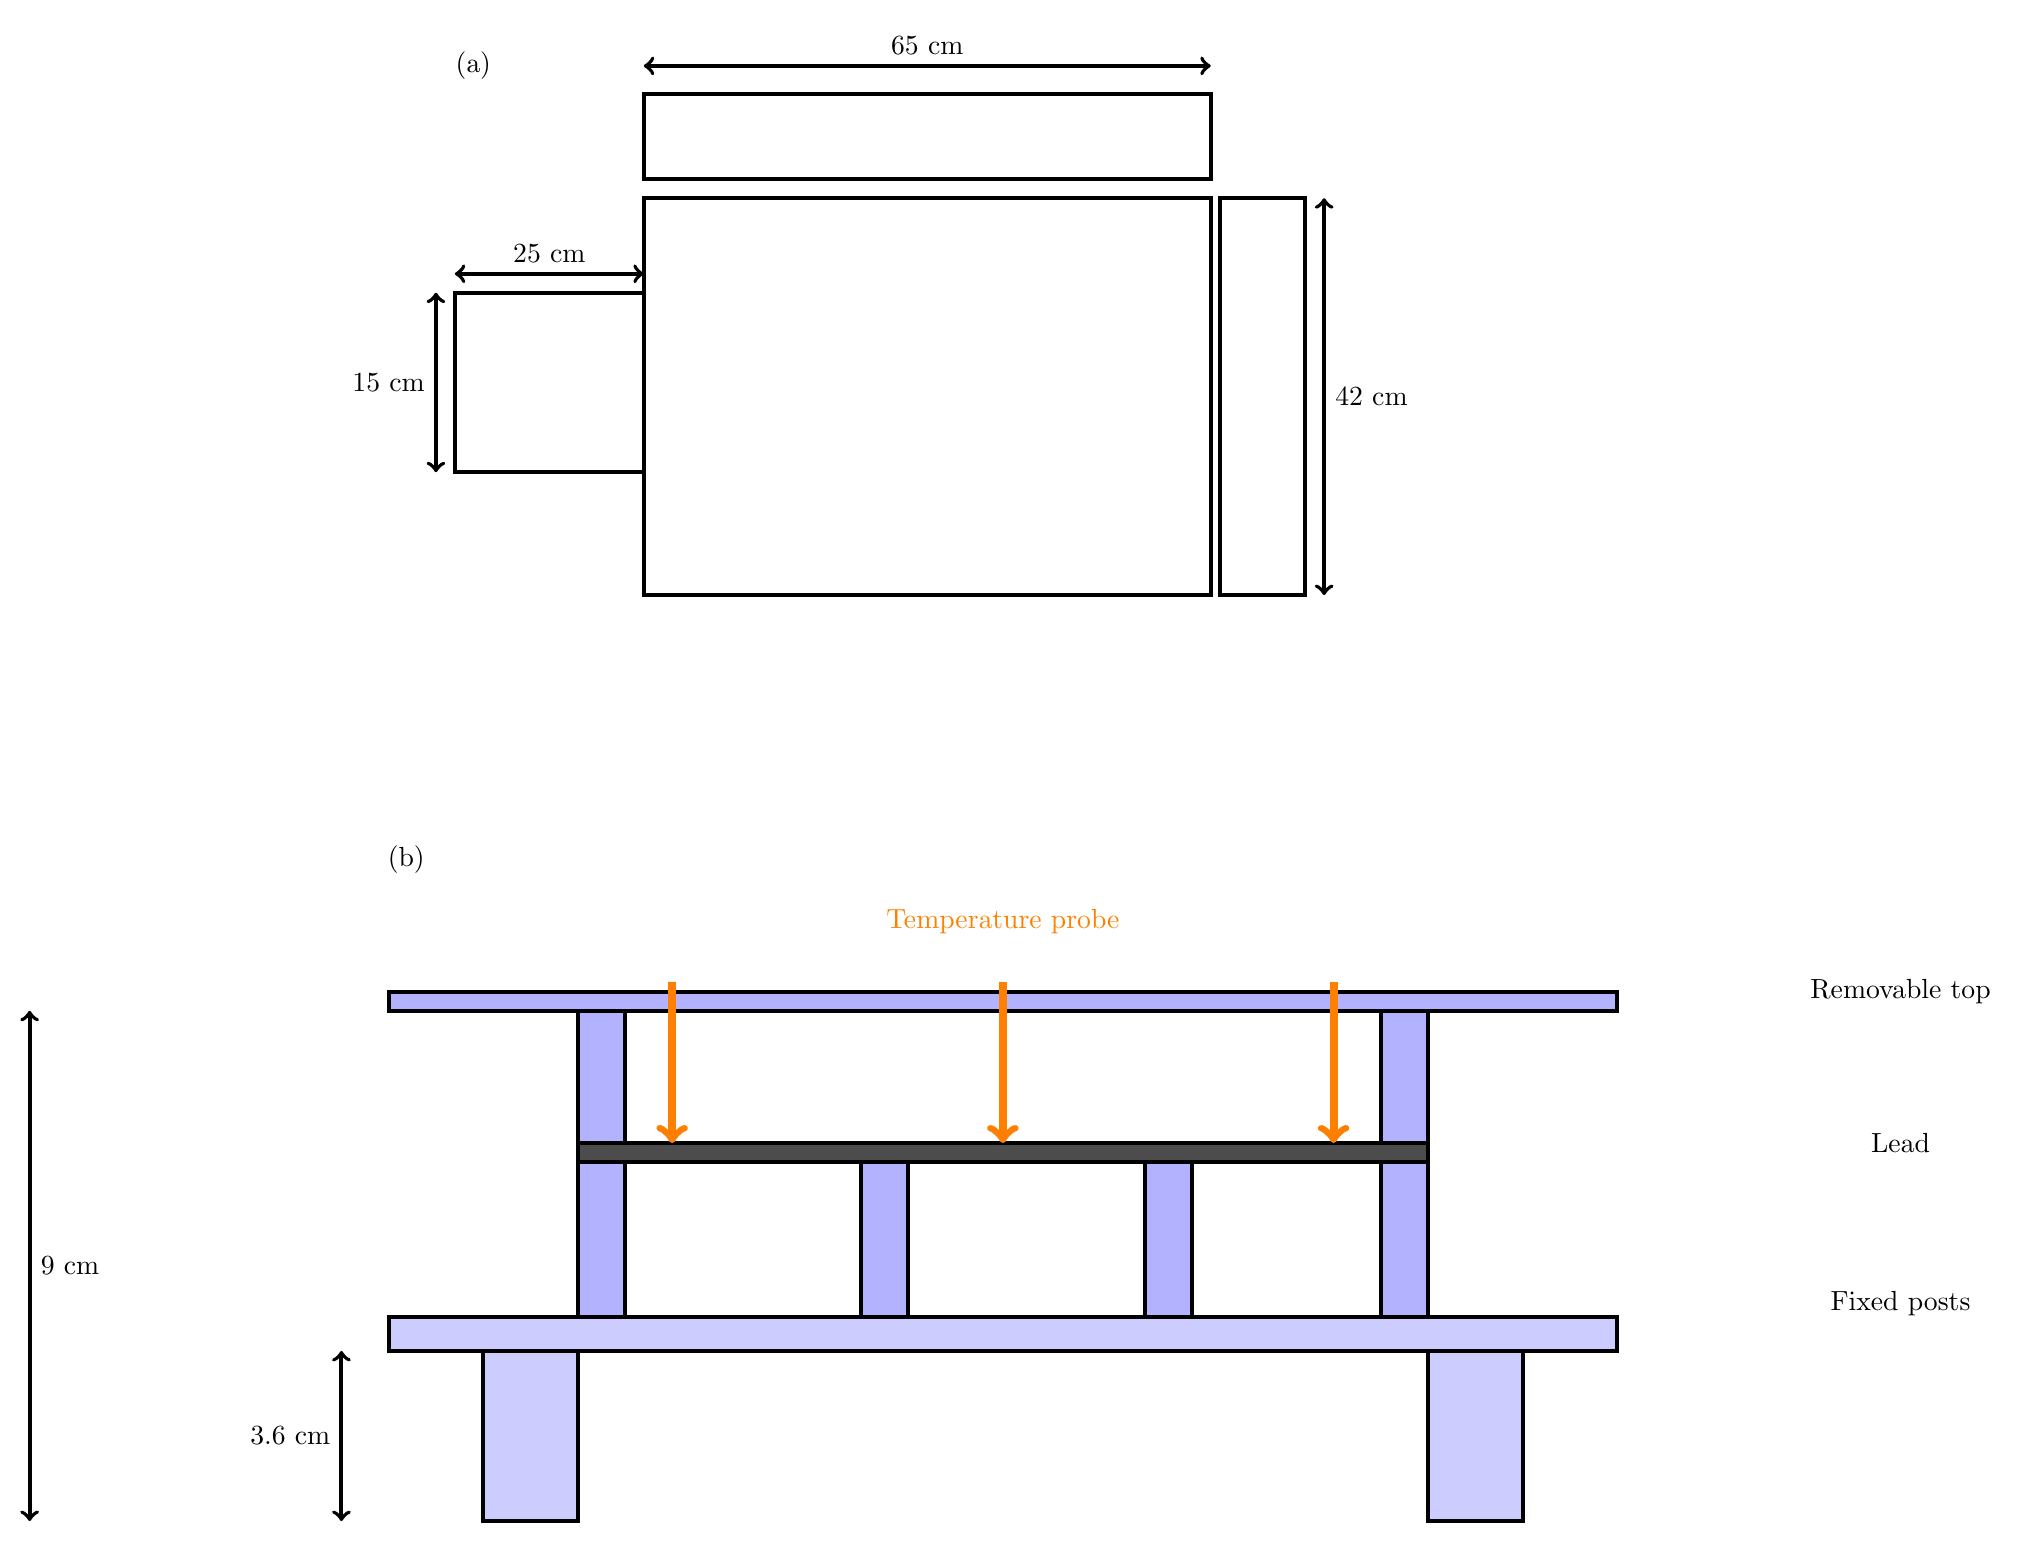
\begin{tikzpicture}[line width=0.5mm, scale=1.2]

% ----------------- (a) Top View -----------------
\node[left] at (0.5, 5.6) {(a)}; % Move label (a) to the left of the figure

% Large horizontal box (centered horizontally)
\draw[black] (2,0) rectangle (8,4.2); % Main rectangle
% Small horizontal box on top
\draw[black] (2,4.4) rectangle (8,5.3); % Slim rectangle (9cm width)
% Vertical rectangle on the right
\draw[black] (8.1,0) rectangle (9,4.2); % Vertical rectangle 42cm tall

% Square cut-out on the left
\draw[black] (0,1.3) rectangle (2,3.2); % Head as a rectangle

% Top dimensions
\draw[<->] (0,3.4) -- (2,3.4) node[midway,above] {25 cm}; % Dimension for the head
\draw[<->] (-0.2,1.3) -- (-0.2,3.2) node[midway,left] {15 cm}; % Vertical dimension for the head
\draw[<->] (9.2,0) -- (9.2,4.2) node[midway,right] {42 cm}; % Dimension for the vertical box
\draw[<->] (2,5.6) -- (8,5.6) node[midway,above] {65 cm}; % Adjusted horizontal dimension

% ----------------- (b) Side View -----------------
\begin{scope}[shift={(-.7,-8)}] % Shift the whole side view below the top view

\node[left] at (0.5, 5.2) {(b)}; % Move label (b) to the left of the figure

% Base of the table (doubled width)
\draw[black,fill=blue!20] (0,0) rectangle (13,0.36); % Base rectangle (3.6 cm tall)

% Shortened Legs below the base
\draw[black,fill=blue!20] (1,-1.8) -- (1,0) -- (2,0) -- (2,-1.8) -- cycle; % Left post
\draw[black,fill=blue!20] (11,-1.8) -- (11,0) -- (12,0) -- (12,-1.8) -- cycle; % Right post

% Fixed posts for the lead
% Two long vertical posts from base to the top
\draw[black,fill=blue!30] (2,0.36) -- (2,3.6) -- (2.5,3.6) -- (2.5,0.36) -- cycle; % Left long post
\draw[black,fill=blue!30] (10.5,0.36) -- (10.5,3.6) -- (11,3.6) -- (11,0.36) -- cycle; % Right long post

% Two short vertical posts from base to the lead
\draw[black,fill=blue!30] (5,0.36) -- (5,2) -- (5.5,2) -- (5.5,0.36) -- cycle; % Left short post
\draw[black,fill=blue!30] (8,0.36) -- (8,2) -- (8.5,2) -- (8.5,0.36) -- cycle; % Right short post

% Lead: Thin slightly longer black rectangle
\draw[black,fill=black!70] (2,2) rectangle (11,2.2); % Thin black rectangle slightly below the midpoint (2 cm)

% Top removable part (shortened distance from base)
\draw[black,fill=blue!30] (0,3.6) rectangle (13,3.8); % Removable top at 9 cm above floor

% Arrows for the temperature probes
% Left arrow
\draw[orange,thick,line width=1mm,->] (3,3.9) -- (3,2.2); 
% Center arrow
\draw[orange,thick,line width=1mm,->] (6.5,3.9) -- (6.5,2.2);
% Right arrow
\draw[orange,thick,line width=1mm,->] (10,3.9) -- (10,2.2);

% Labels for the temperature probes (moved to top)
\node[orange,align=center,above] at (6.5,4.3) {Temperature probe};

% Labels for each component
\node[align=left] at (16,3.8) {Removable top};
\node[align=left] at (16,0.5) {Fixed posts};
\node[align=left] at (16,2.2) {Lead};
%\node[align=left] at (14,0.5) {Base};
%\node[align=left] at (14,-1.5) {Legs};

% Dimension arrows for side view
\draw[<->] (-0.5,-1.8) -- (-0.5,0) node[midway,left] {3.6 cm}; % New shorter leg dimension
\draw[<->] (-3.8,-1.8) -- (-3.8,3.6) node[midway,right] {9 cm}; % Distance from floor to top

\end{scope}
\end{tikzpicture}